\documentclass[tikz, border=10pt]{standalone}
\usetikzlibrary{shapes.geometric, arrows.meta, positioning, calc, decorations.pathmorphing, matrix}
\usepackage{amsmath, amssymb}
\usepackage{xcolor}

\definecolor{panelbg}{RGB}{245, 247, 250}
\definecolor{panelborder}{RGB}{200, 210, 220}
\definecolor{carrierred}{RGB}{220, 50, 32}
\definecolor{latticeblue}{RGB}{0, 114, 178}
\definecolor{laserorange}{RGB}{230, 120, 20}

\begin{document}

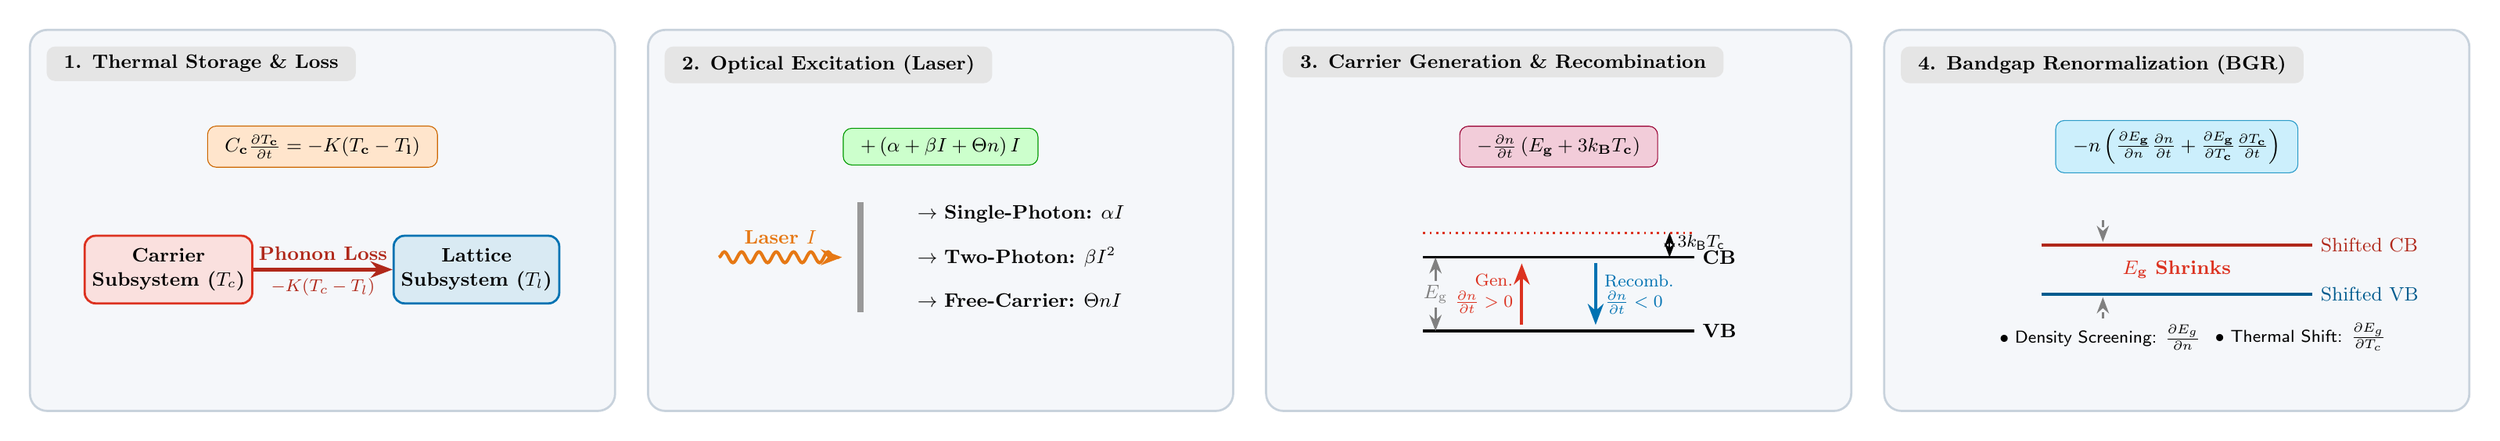
\begin{tikzpicture}[
    >=Stealth,
    font=\sffamily,
    panel/.style={
        fill=panelbg,
        draw=panelborder,
        line width=1pt,
        rounded corners=8pt,
        inner sep=10pt,
        minimum width=9.5cm,
        minimum height=6.2cm,
        align=center
    },
    titlebox/.style={
        draw=none,
        fill=gray!20,
        rounded corners=4pt,
        font=\bfseries\small,
        inner xsep=8pt,
        inner ysep=4pt
    },
    subbox/.style={
        draw,
        rectangle,
        rounded corners=5pt,
        minimum width=2.4cm,
        minimum height=1.1cm,
        align=center,
        font=\small\bfseries,
        line width=1pt
    }
]


% =========================================================================
    % 1x4 PANEL MATRIX (SINGLE ROW)
    % =========================================================================
    \matrix (m) [matrix of nodes, nodes in empty cells, column sep=0.5cm] {
        % Row 1: Panels 1, 2, 3, 4
        \node[panel] (p1) {}; & \node[panel] (p2) {}; & \node[panel] (p3) {}; & \node[panel] (p4) {}; \\
    };

    % -------------------------------------------------------------------------
    % PANEL 1: THERMAL STORAGE & LOSS
    % -------------------------------------------------------------------------
    \node[titlebox, anchor=north west] at (p1.north west) [xshift=8pt, yshift=-8pt] {1. Thermal Storage \& Loss};
    \node[titlebox, fill=orange!20, draw=orange!80!black] (p1_eq) at ([yshift=1.2cm]p1.center) {
        $C_{\text{c}}\frac{\partial T_{\text{c}}}{\partial t} = -K(T_{\text{c}} - T_{\text{l}})$
    };
    \node[subbox, fill=carrierred!15, draw=carrierred] (carrier_box) at ([xshift=-2.5cm, yshift=-0.8cm]p1.center) {
        Carrier\\Subsystem ($T_c$)
    };
    \node[subbox, fill=latticeblue!15, draw=latticeblue] (lattice_box) at ([xshift=2.5cm, yshift=-0.8cm]p1.center) {
        Lattice\\Subsystem ($T_l$)
    };
    \draw[->, line width=1.6pt, carrierred!80!black] (carrier_box) -- (lattice_box)
        node[midway, above, font=\small\bfseries] {Phonon Loss}
        node[midway, below, font=\footnotesize] {$-K(T_c - T_l)$};

    % -------------------------------------------------------------------------
    % PANEL 2: OPTICAL EXCITATION (LASER)
    % -------------------------------------------------------------------------
    \node[titlebox, anchor=north west] at (p2.north west) [xshift=8pt, yshift=-8pt] {2. Optical Excitation (Laser)};
    \node[titlebox, fill=green!20, draw=green!60!black] (p2_eq) at ([yshift=1.2cm]p2.center) {
        $+\left(\alpha + \beta I + \Theta n\right)I$
    };
    
    \node[anchor=west, font=\small] (abs1) at ([xshift=-0.5cm, yshift=0.1cm]p2.center) {$\rightarrow$ \textbf{Single-Photon:} $\alpha I$};
    \node[anchor=west, font=\small] (abs2) at ([xshift=-0.5cm, yshift=-0.6cm]p2.center) {$\rightarrow$ \textbf{Two-Photon:} $\beta I^2$};
    \node[anchor=west, font=\small] (abs3) at ([xshift=-0.5cm, yshift=-1.3cm]p2.center) {$\rightarrow$ \textbf{Free-Carrier:} $\Theta n I$};

    \draw[->, line width=1.5pt, laserorange, decorate, decoration={snake, amplitude=2.5pt, segment length=8pt}] 
        ([xshift=-3.6cm, yshift=-0.6cm]p2.center) -- ([xshift=-1.6cm, yshift=-0.6cm]p2.center) 
        node[midway, above=2pt, font=\small\bfseries] {Laser $I$};

    \draw[line width=3pt, gray!80] ([xshift=-1.3cm, yshift=0.3cm]p2.center) -- ([xshift=-1.3cm, yshift=-1.5cm]p2.center);

    % -------------------------------------------------------------------------
    % PANEL 3: CARRIER GENERATION & RECOMBINATION
    % -------------------------------------------------------------------------
    \node[titlebox, anchor=north west] at (p3.north west) [xshift=8pt, yshift=-8pt] {3. Carrier Generation \& Recombination};
    \node[titlebox, fill=purple!20, draw=purple!80!black] (p3_eq) at ([yshift=1.2cm]p3.center) {
        $-\frac{\partial n}{\partial t}\left(E_{\text{g}} + 3k_{\text{B}}T_{\text{c}}\right)$
    };

    \coordinate (b3) at ([yshift=-0.6cm]p3.center);
    \draw[line width=1.2pt] ([xshift=-2.2cm]b3) -- ([xshift=2.2cm]b3) node[right, font=\small\bfseries] {CB};
    \draw[line width=1.2pt] ([xshift=-2.2cm, yshift=-1.2cm]b3) -- ([xshift=2.2cm, yshift=-1.2cm]b3) node[right, font=\small\bfseries] {VB};

    \draw[<->, line width=1pt, gray] ([xshift=-2cm, yshift=-1.2cm]b3) -- ([xshift=-2cm]b3)
        node[midway, fill=panelbg, inner sep=2pt, font=\small] {$E_{\text{g}}$};

    \draw[->, line width=1.5pt, carrierred] ([xshift=-0.6cm, yshift=-1.1cm]b3) -- ([xshift=-0.6cm, yshift=-0.1cm]b3)
        node[midway, left, font=\footnotesize, align=right] {Gen.\\$\frac{\partial n}{\partial t} > 0$};

    \draw[->, line width=1.5pt, latticeblue] ([xshift=0.6cm, yshift=-0.1cm]b3) -- ([xshift=0.6cm, yshift=-1.1cm]b3)
        node[midway, right, font=\footnotesize, align=left] {Recomb.\\$\frac{\partial n}{\partial t} < 0$};

    \draw[dotted, line width=1pt, carrierred] ([xshift=-2.2cm, yshift=0.4cm]b3) -- ([xshift=2.2cm, yshift=0.4cm]b3);
    \draw[<->, line width=0.8pt] ([xshift=1.8cm]b3) -- ([xshift=1.8cm, yshift=0.4cm]b3)
        node[midway, right, yshift=1, font=\footnotesize\sffamily] {$3k_{\text{B}}T_{\text{c}}$};

    % -------------------------------------------------------------------------
    % PANEL 4: BANDGAP RENORMALIZATION
    % -------------------------------------------------------------------------
    \node[titlebox, anchor=north west] at (p4.north west) [xshift=8pt, yshift=-8pt] {4. Bandgap Renormalization (BGR)};
    \node[titlebox, fill=cyan!20, draw=cyan!80!black] (p4_eq) at ([yshift=1.2cm]p4.center) {
        $-n\left(\frac{\partial E_{\text{g}}}{\partial n}\frac{\partial n}{\partial t} + \frac{\partial E_{\text{g}}}{\partial T_{\text{c}}}{\frac{\partial T_{\text{c}}}{\partial t}}\right)$
    };

    \coordinate (b4) at ([yshift=-0.2cm]p4.center);
    \draw[line width=1.2pt, carrierred!80!black] ([xshift=-2.2cm, yshift=-0.2cm]b4) -- ([xshift=2.2cm, yshift=-0.2cm]b4) node[right, font=\small] {Shifted CB};
    \draw[line width=1.2pt, latticeblue!80!black] ([xshift=-2.2cm, yshift=-1.0cm]b4) -- ([xshift=2.2cm, yshift=-1.0cm]b4) node[right, font=\small] {Shifted VB};

    \draw[->, line width=1pt, dashed, gray] ([xshift=-1.2cm, yshift=0.2cm]b4) -- ([xshift=-1.2cm, yshift=-0.15cm]b4);
    \draw[->, line width=1pt, dashed, gray] ([xshift=-1.2cm, yshift=-1.4cm]b4) -- ([xshift=-1.2cm, yshift=-1.05cm]b4);

    \node[font=\small\bfseries, carrierred] at ([yshift=-0.6cm]b4) {$E_{\text{g}}$ Shrinks};

    \node[anchor=west, font=\footnotesize\sffamily] at ([xshift=-3cm, yshift=-1.7cm]b4) {$\bullet$ Density Screening: $\frac{\partial E_g}{\partial n}$};
    \node[anchor=west, font=\footnotesize\sffamily] at ([xshift=0.5cm, yshift=-1.7cm]b4) {$\bullet$ Thermal Shift: $\frac{\partial E_g}{\partial T_c}$};

\end{tikzpicture}

\end{document}
